\documentclass{article}
\usepackage{tikz}
\usetikzlibrary{calc}
\usetikzlibrary{shapes.geometric, arrows, positioning, decorations.pathreplacing}

\begin{document}

\begin{figure}[ht]
\centering
\begin{tikzpicture}[node distance=2cm and 2cm, auto]

\foreach \x in {1,...,12}
{
  \ifnum\x<5
    \def\rectColor{green}
  \else
    \ifnum\x<9
    \def\rectColor{blue}
  \else
    \def\rectColor{orange}
  \fi
    \fi
  \node[yslant=0.5, fill=\rectColor, opacity=0.8] (wsi\x) at (\x-6,0) 
  {\includegraphics[width=.1\textwidth, height=.1\textheight]{./wsi\x.png}};
}


\draw[decorate, decoration={brace, amplitude=10pt, mirror}]
    (-6,-1.5) -- (6.5,-1.5) node [midway, below=10pt] (Train) {Training data} ;
% ([shift={(-1.5,0.3+\shiftY)}]csBase) 

\node [draw, diamond, aspect=2, below=1cm of Train] (CS) {Use conditional sampling?};
\draw[->] (Train) edge (CS);


%% conditional sampling
\def\shiftX{0.5};
\def\shiftY{-2};
% \coordinate (csBase) at (7,2);
% \coordinate [below=3.5cm of CS, right=2cm of CS] (csBase) {};
\coordinate [below=of CS, right=4] (csBase) {};
\coordinate [below=of CS, left=5] (rBase) {};

\foreach \y in {1,...,3}
{
    \begin{scope}[yshift=\y*\shiftY]
        \foreach \x in {1,...,2}
        {
          \ifnum\y<2
            \def\rectColor{green}
          \else
            \ifnum\y<3
            \def\rectColor{blue}
          \else
            \def\rectColor{orange}
          \fi
            \fi
            \pgfmathsetmacro\wsiName{int((\x-1)*\y+\x)}
            \node[yslant=0.5, fill=\rectColor] (cswsi\y\x) at ([shift={(\x*\shiftX,\y*\shiftY)}]csBase) 
            {
              {\includegraphics[width=.05\textwidth, height=.05\textheight]{./wsi\wsiName.png}}
        };
        }

          \ifnum\y<2
            \node[yslant=0.5, fill=orange] (cswsi\y3) at ([shift={(2*\shiftX+0.5,\y*\shiftY)}]csBase) 
            {
              {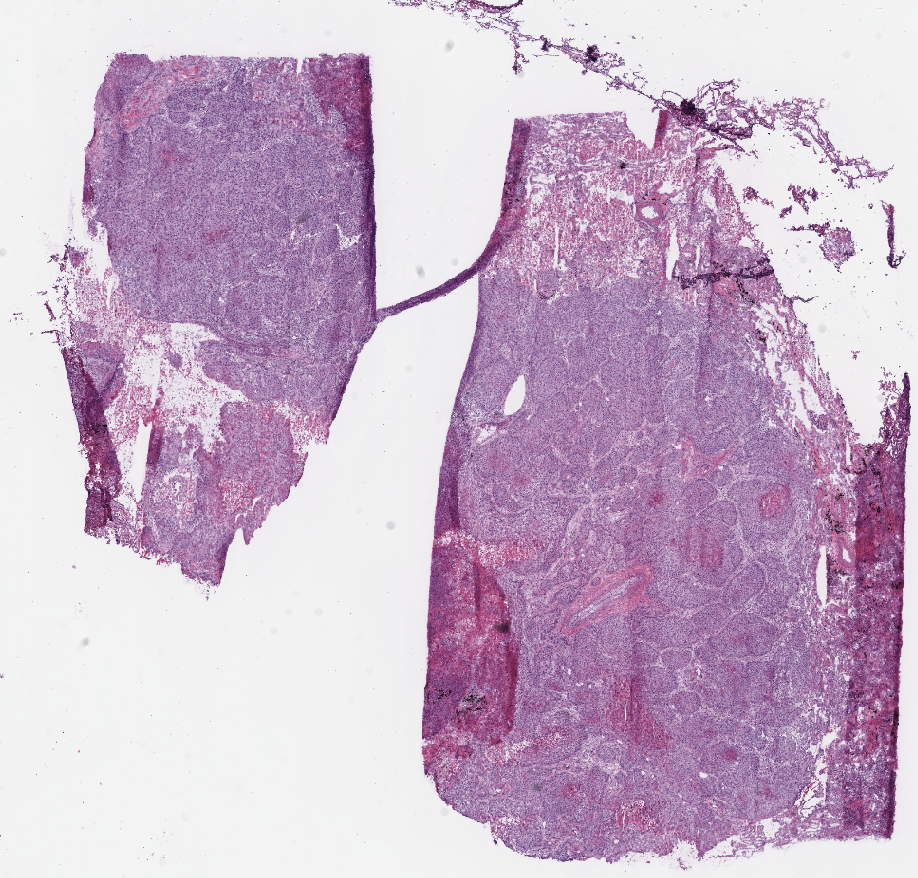
\includegraphics[width=.05\textwidth, height=.05\textheight]{./wsi5.png}}
        };
            \node[yslant=0.5, fill=blue] (cswsi\y4) at ([shift={(2*\shiftX+1,\y*\shiftY)}]csBase) 
            {
              {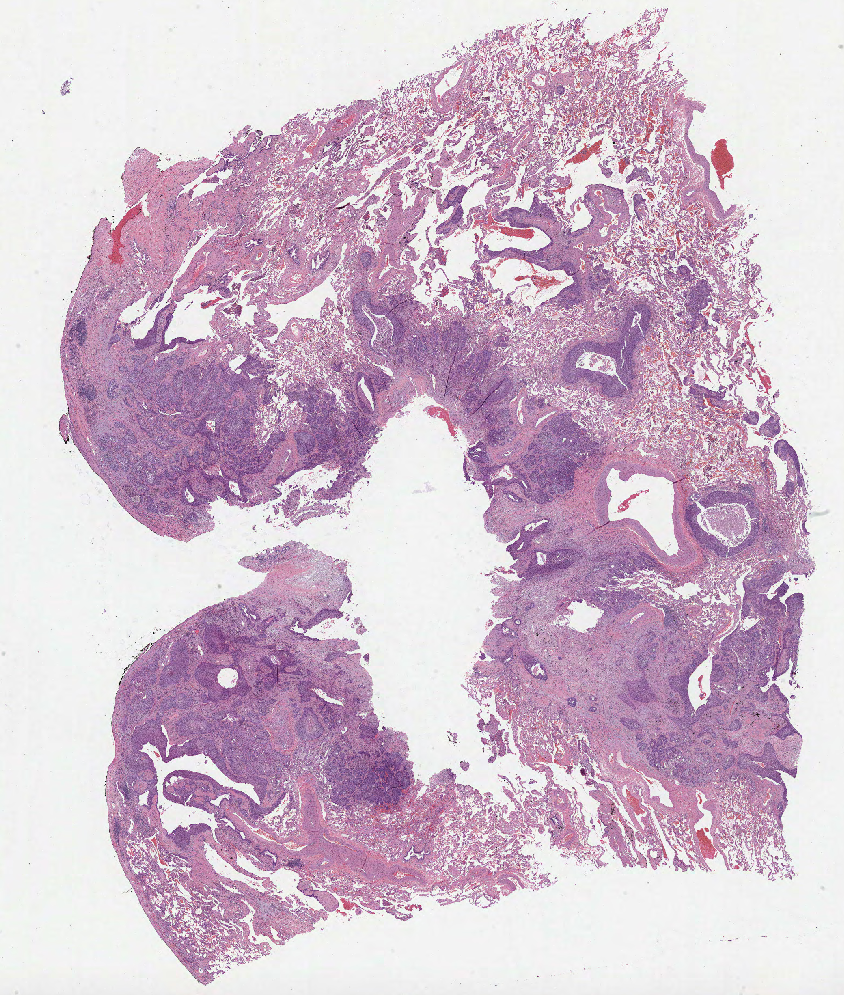
\includegraphics[width=.05\textwidth, height=.05\textheight]{./wsi3.png}}
        };
          \else
            \ifnum\y<3
            \node[yslant=0.5, fill=green] (cswsi\y3) at ([shift={(2*\shiftX+0.5,\y*\shiftY)}]csBase) 
            {
              {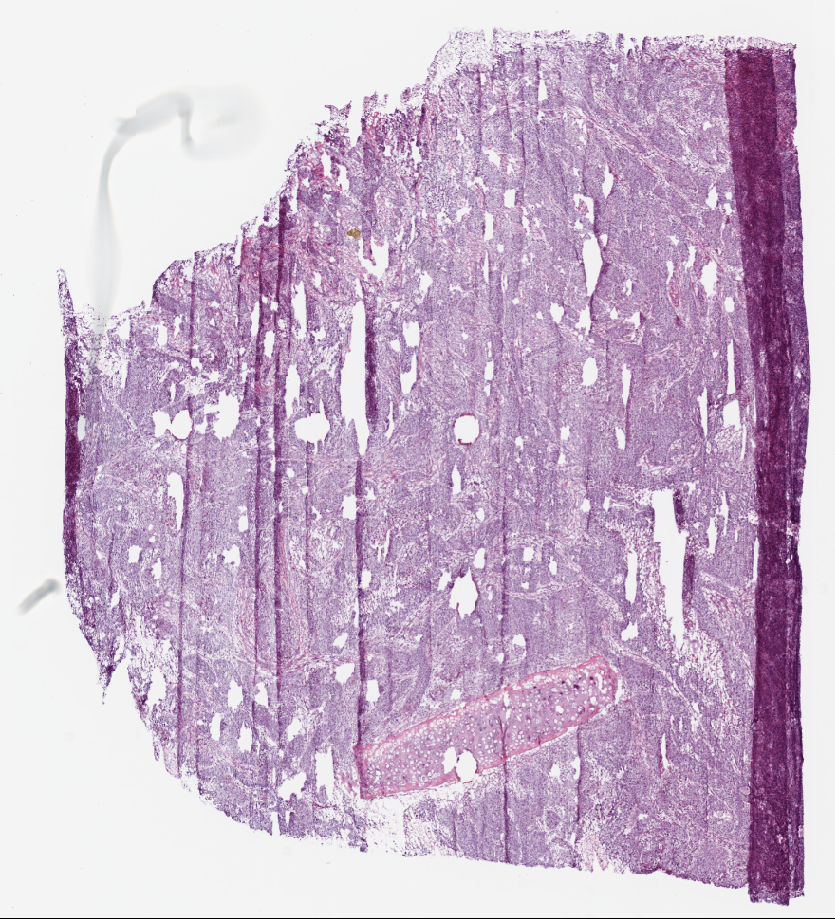
\includegraphics[width=.05\textwidth, height=.05\textheight]{./wsi2.png}}
        };
            \node[yslant=0.5, fill=orange] (cswsi\y4) at ([shift={(2*\shiftX+1,\y*\shiftY)}]csBase) 
            {
              {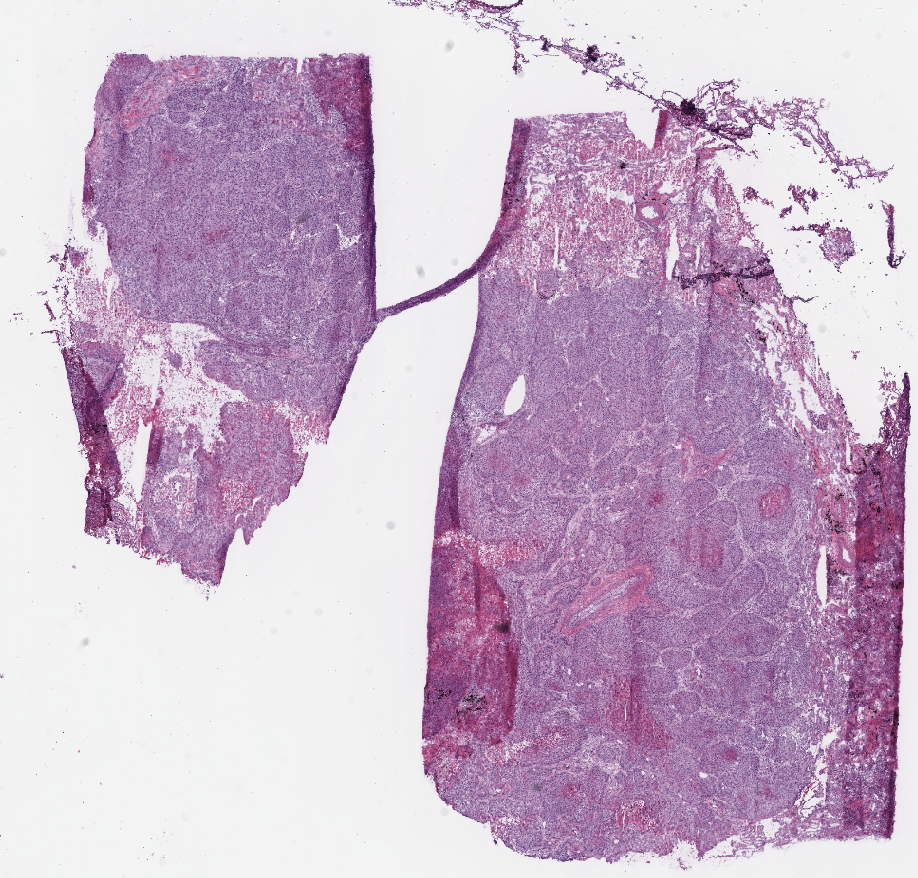
\includegraphics[width=.05\textwidth, height=.05\textheight]{./wsi5.png}}
        };
          \else
            \node[yslant=0.5, fill=green] (cswsi\y3) at ([shift={(2*\shiftX+0.5,\y*\shiftY)}]csBase) 
            {
              {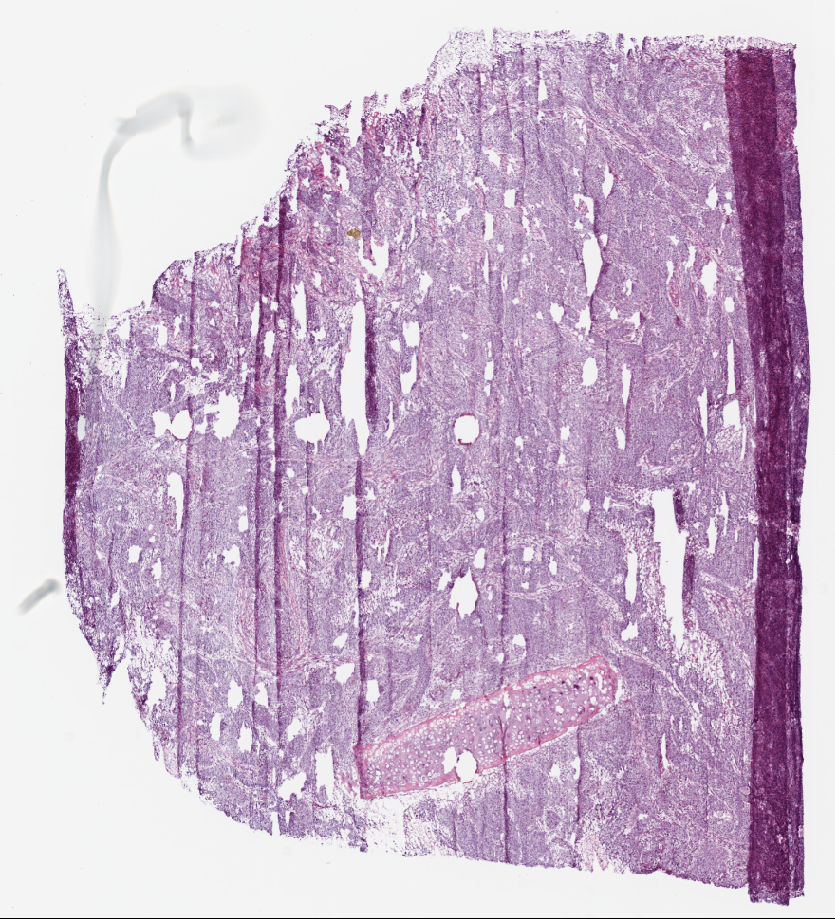
\includegraphics[width=.05\textwidth, height=.05\textheight]{./wsi2.png}}
        };
            \node[yslant=0.5, fill=blue] (cswsi\y4) at ([shift={(2*\shiftX+1,\y*\shiftY)}]csBase) 
            {
              {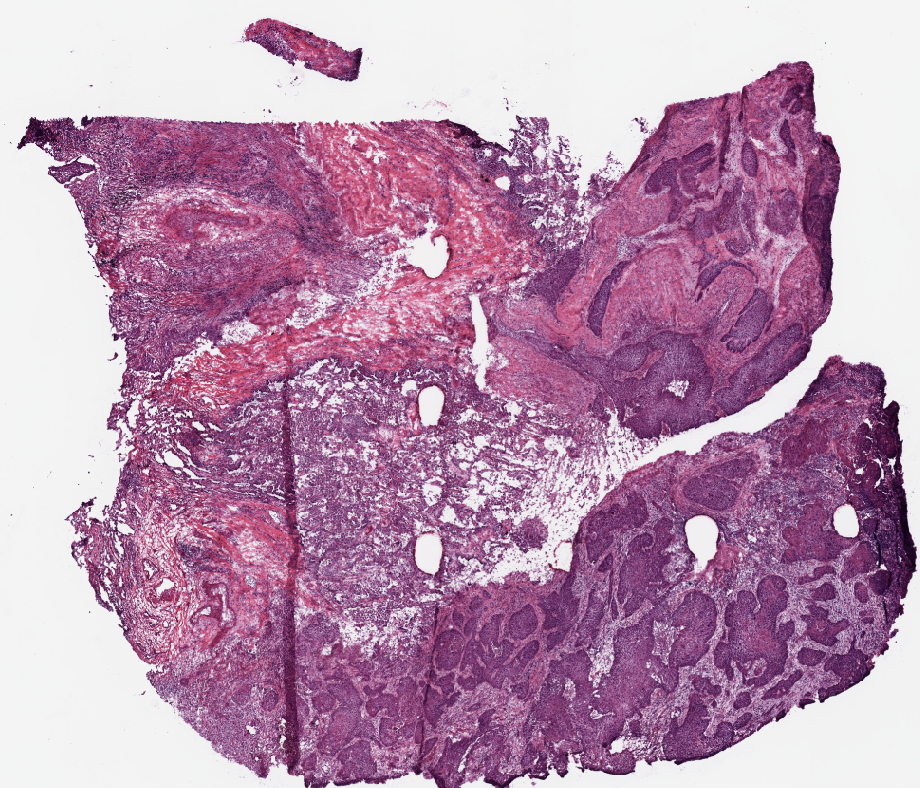
\includegraphics[width=.05\textwidth, height=.05\textheight]{./wsi4.png}}
        };
          \fi
          \fi
        \draw (cswsi\y1.south west) rectangle (cswsi\y4.north east) ;
        \node[anchor=north] at ([shift={(-0.8,0.5)}]cswsi\y1.west) {Batch \number\numexpr\y\relax};
    \end{scope}
}


\foreach \y in {1,...,3}
{
    \begin{scope}[yshift=\y*\shiftY]
          \ifnum\y<2
            \node[yslant=0.5, fill=green] (cswsi\y1) at ([shift={(1*\shiftX+0.5,\y*\shiftY)}]rBase) 
            {
              {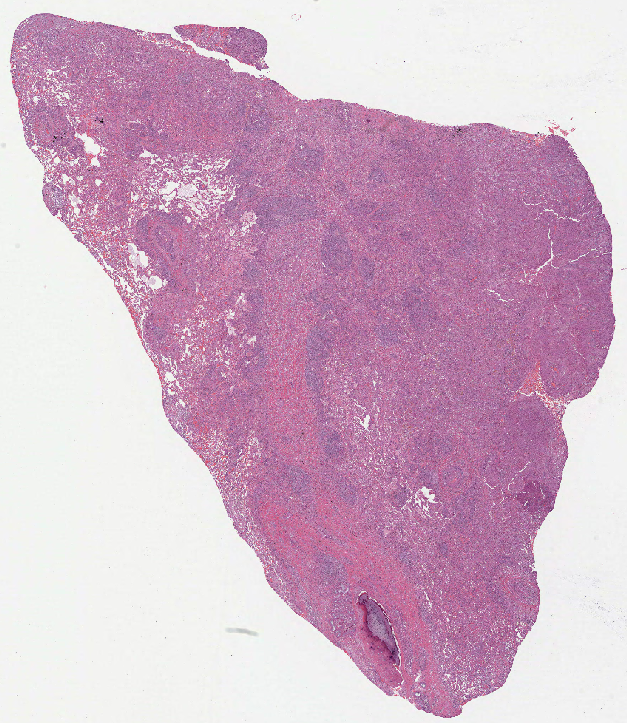
\includegraphics[width=.05\textwidth, height=.05\textheight]{./wsi1.png}}
            };
            \node[yslant=0.5, fill=green] (cswsi\y2) at ([shift={(2*\shiftX+0.5,\y*\shiftY)}]rBase) 
            {
              {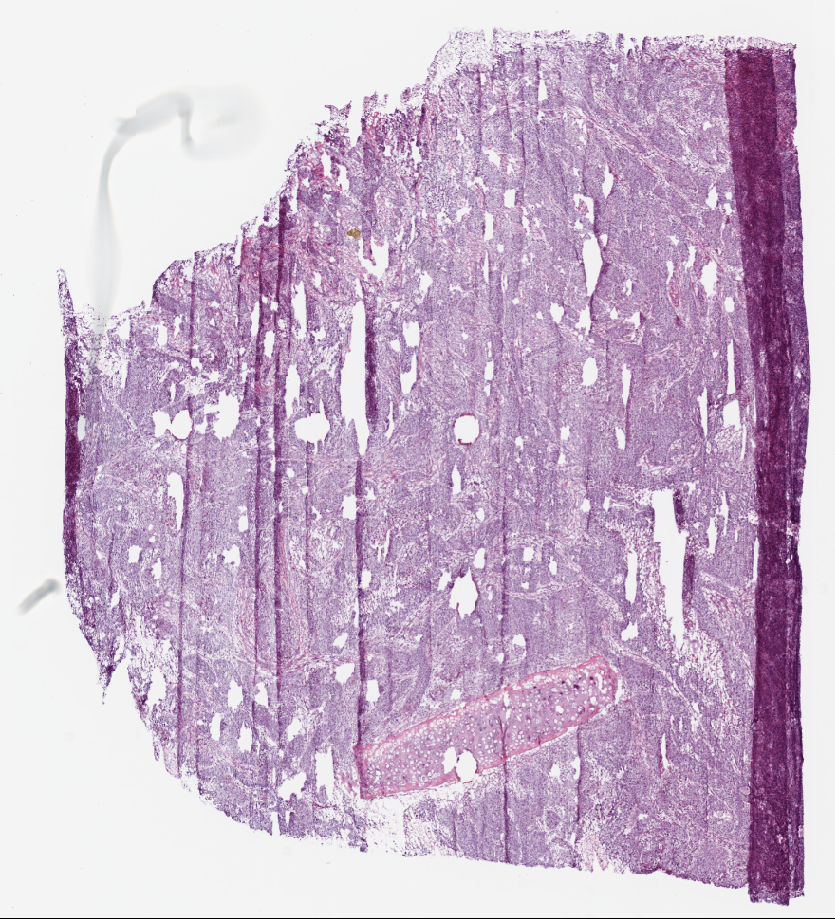
\includegraphics[width=.05\textwidth, height=.05\textheight]{./wsi2.png}}
            };
            \node[yslant=0.5, fill=green] (cswsi\y3) at ([shift={(3*\shiftX+0.5,\y*\shiftY)}]rBase) 
            {
              {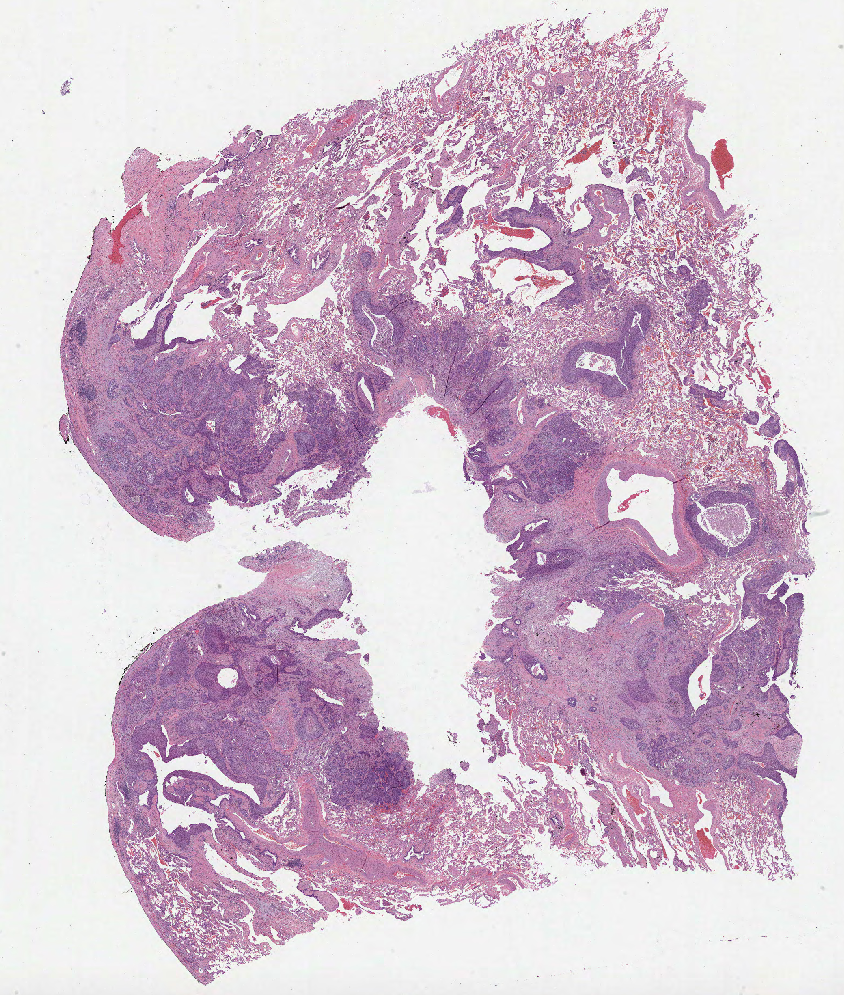
\includegraphics[width=.05\textwidth, height=.05\textheight]{./wsi3.png}}
            };
            \node[yslant=0.5, fill=orange] (cswsi\y4) at ([shift={(4*\shiftX+0.5,\y*\shiftY)}]rBase) 
            {
              {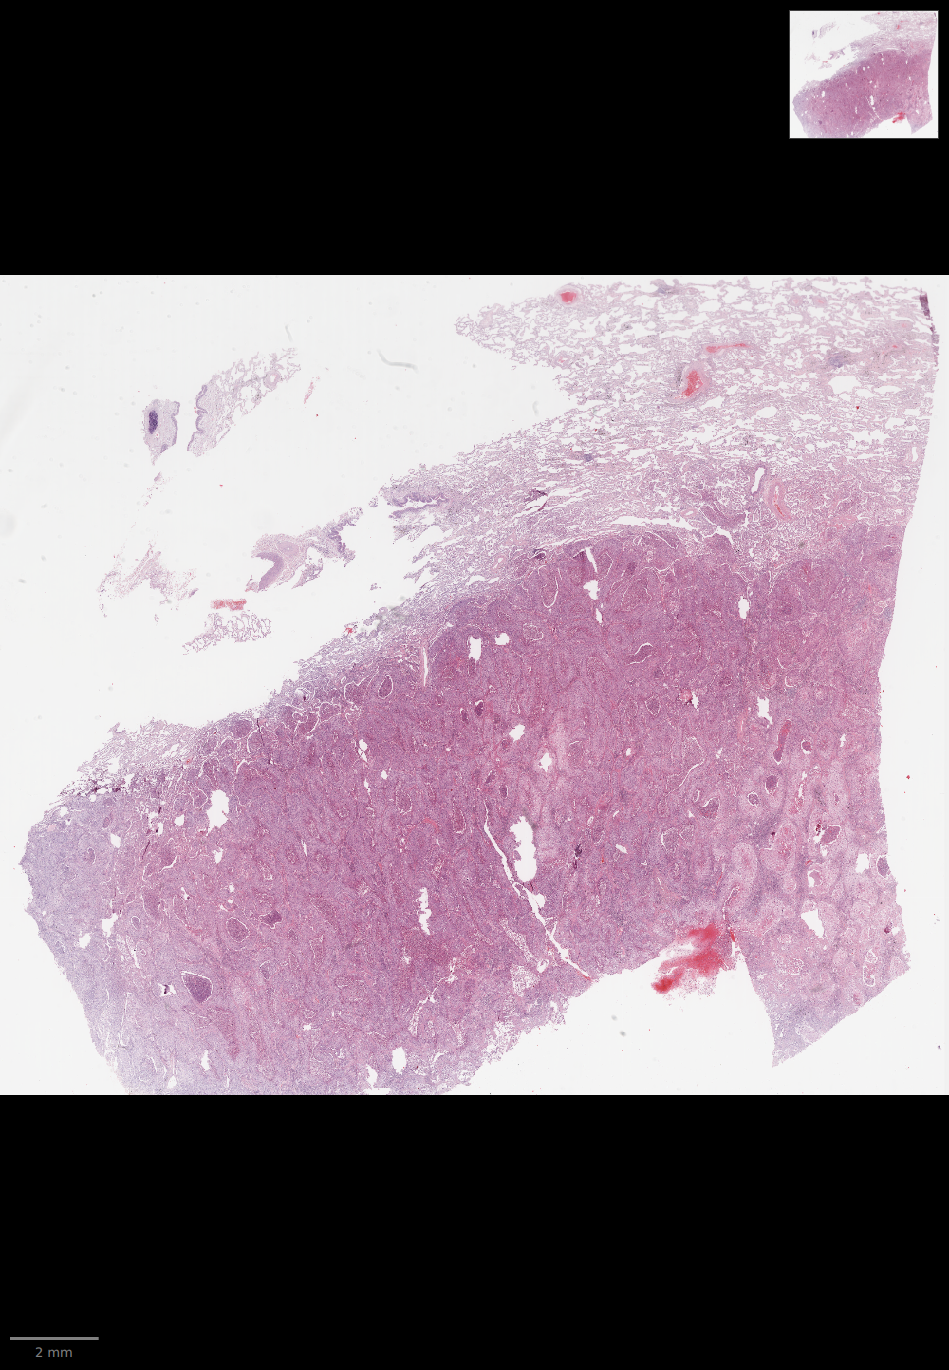
\includegraphics[width=.05\textwidth, height=.05\textheight]{./wsi7.png}}
            };
        \draw (cswsi\y1.south west) rectangle (cswsi\y4.north east) ;
        \node[anchor=north] at ([shift={(-0.8,0.5)}]cswsi\y1.west) {Batch \number\numexpr\y\relax};
        \else
          \ifnum\y<3
            \node[yslant=0.5, fill=blue] (cswsi\y1) at ([shift={(1*\shiftX+0.5,\y*\shiftY)}]rBase) 
            {
              {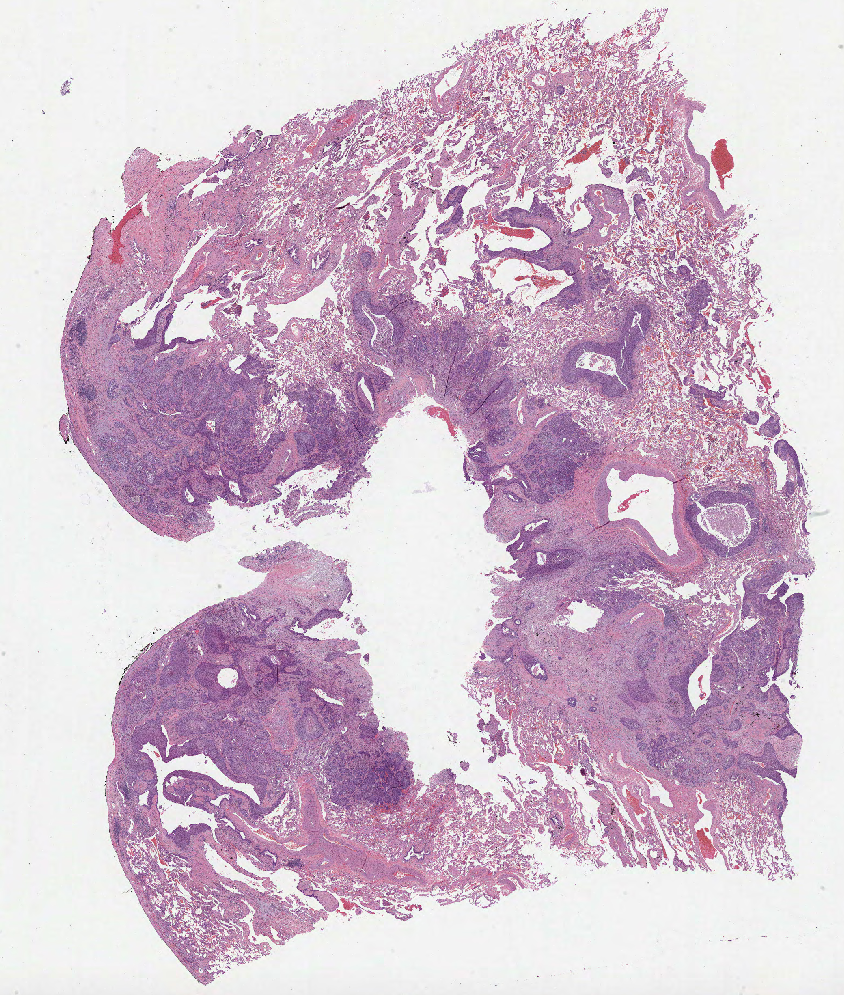
\includegraphics[width=.05\textwidth, height=.05\textheight]{./wsi3.png}}
            };
            \node[yslant=0.5, fill=orange] (cswsi\y2) at ([shift={(2*\shiftX+0.5,\y*\shiftY)}]rBase) 
            {
              {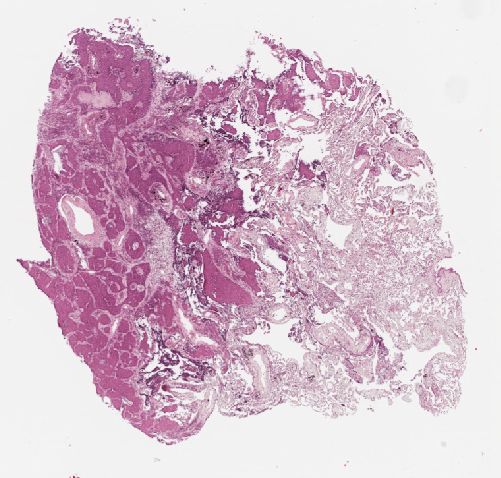
\includegraphics[width=.05\textwidth, height=.05\textheight]{./wsi8.png}}
            };
            \node[yslant=0.5, fill=blue] (cswsi\y3) at ([shift={(3*\shiftX+0.5,\y*\shiftY)}]rBase) 
            {
              {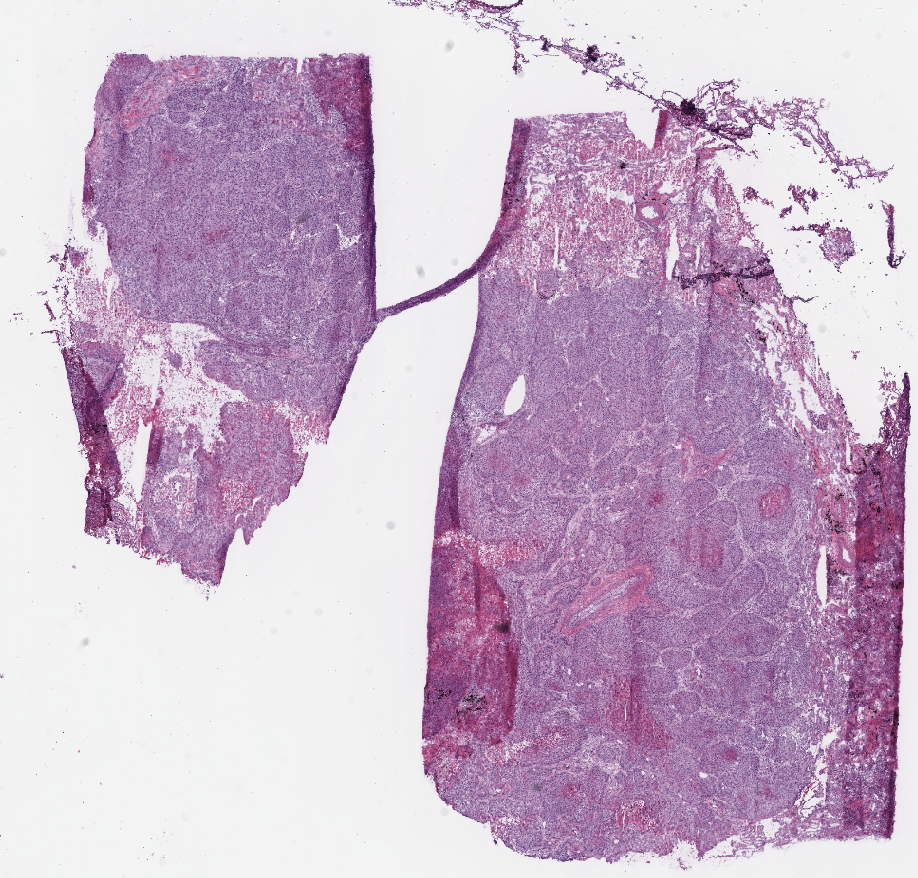
\includegraphics[width=.05\textwidth, height=.05\textheight]{./wsi5.png}}
            };
            \node[yslant=0.5, fill=orange] (cswsi\y4) at ([shift={(4*\shiftX+0.5,\y*\shiftY)}]rBase) 
            {
              {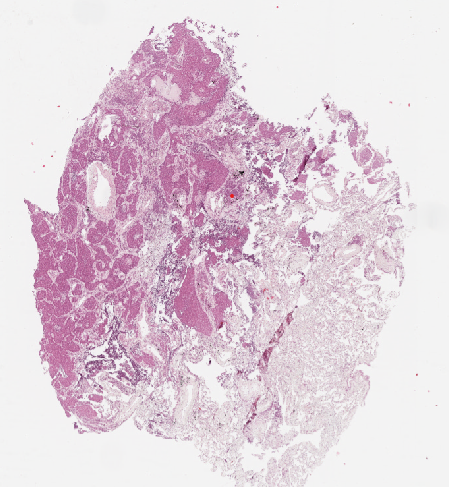
\includegraphics[width=.05\textwidth, height=.05\textheight]{./wsi9.png}}
            };
            \draw (cswsi\y1.south west) rectangle (cswsi\y4.north east) ;
            \node[anchor=north] at ([shift={(-0.8,0.5)}]cswsi\y1.west) {Batch \number\numexpr\y\relax};
        \else
            \node[yslant=0.5, fill=green] (cswsi\y1) at ([shift={(1*\shiftX+0.5,\y*\shiftY)}]rBase) 
            {
              {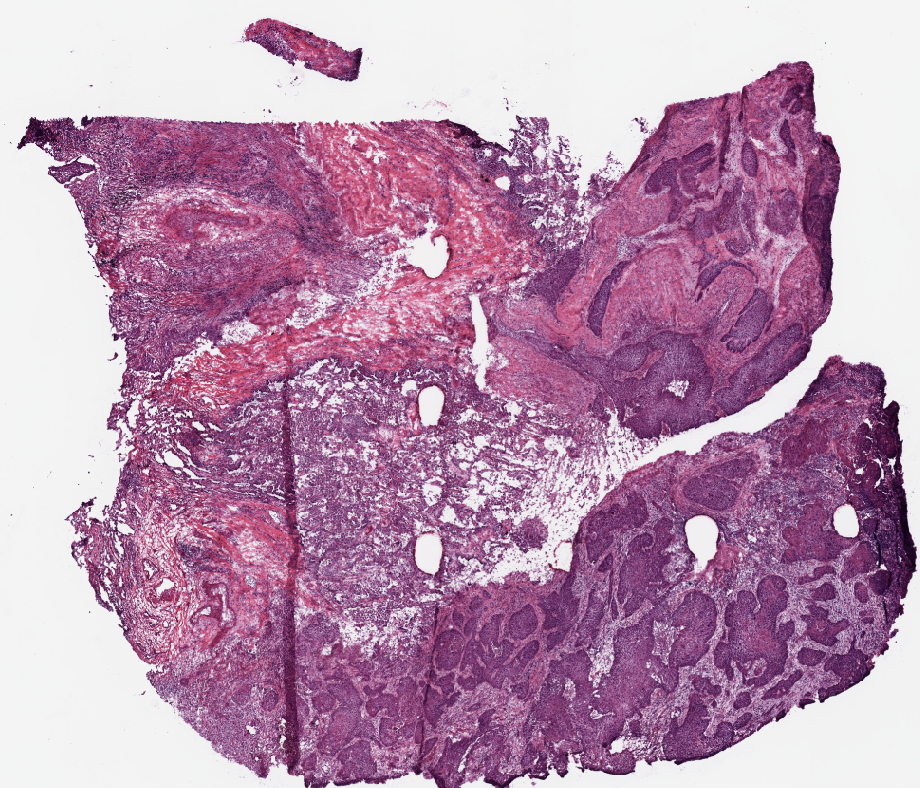
\includegraphics[width=.05\textwidth, height=.05\textheight]{./wsi4.png}}
            };
            \node[yslant=0.5, fill=orange] (cswsi\y2) at ([shift={(2*\shiftX+0.5,\y*\shiftY)}]rBase) 
            {
              {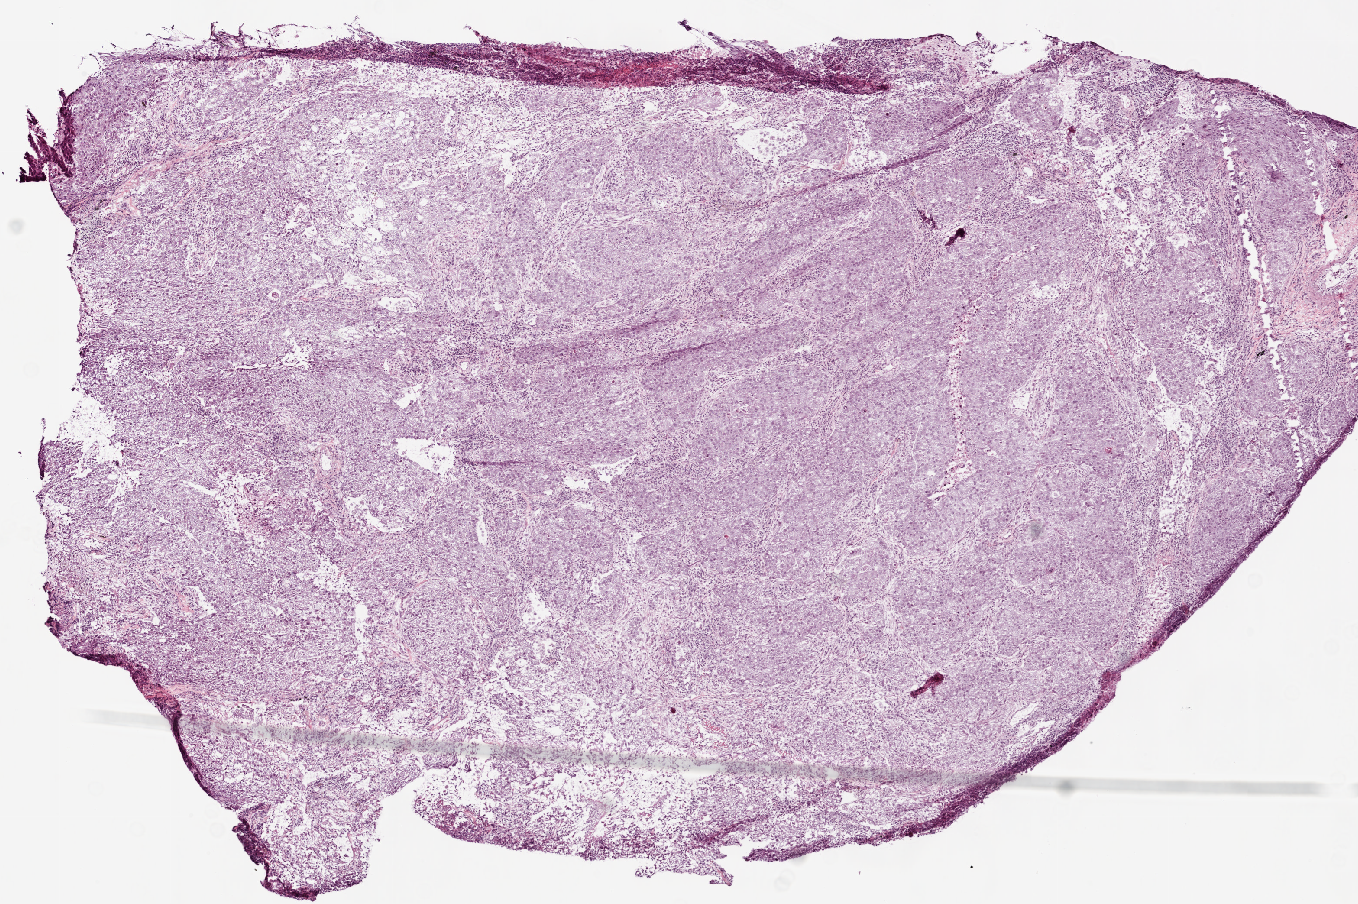
\includegraphics[width=.05\textwidth, height=.05\textheight]{./wsi12.png}}
            };
            \node[yslant=0.5, fill=blue] (rwsi\y3) at ([shift={(3*\shiftX+0.5,\y*\shiftY)}]rBase) 
            {
              {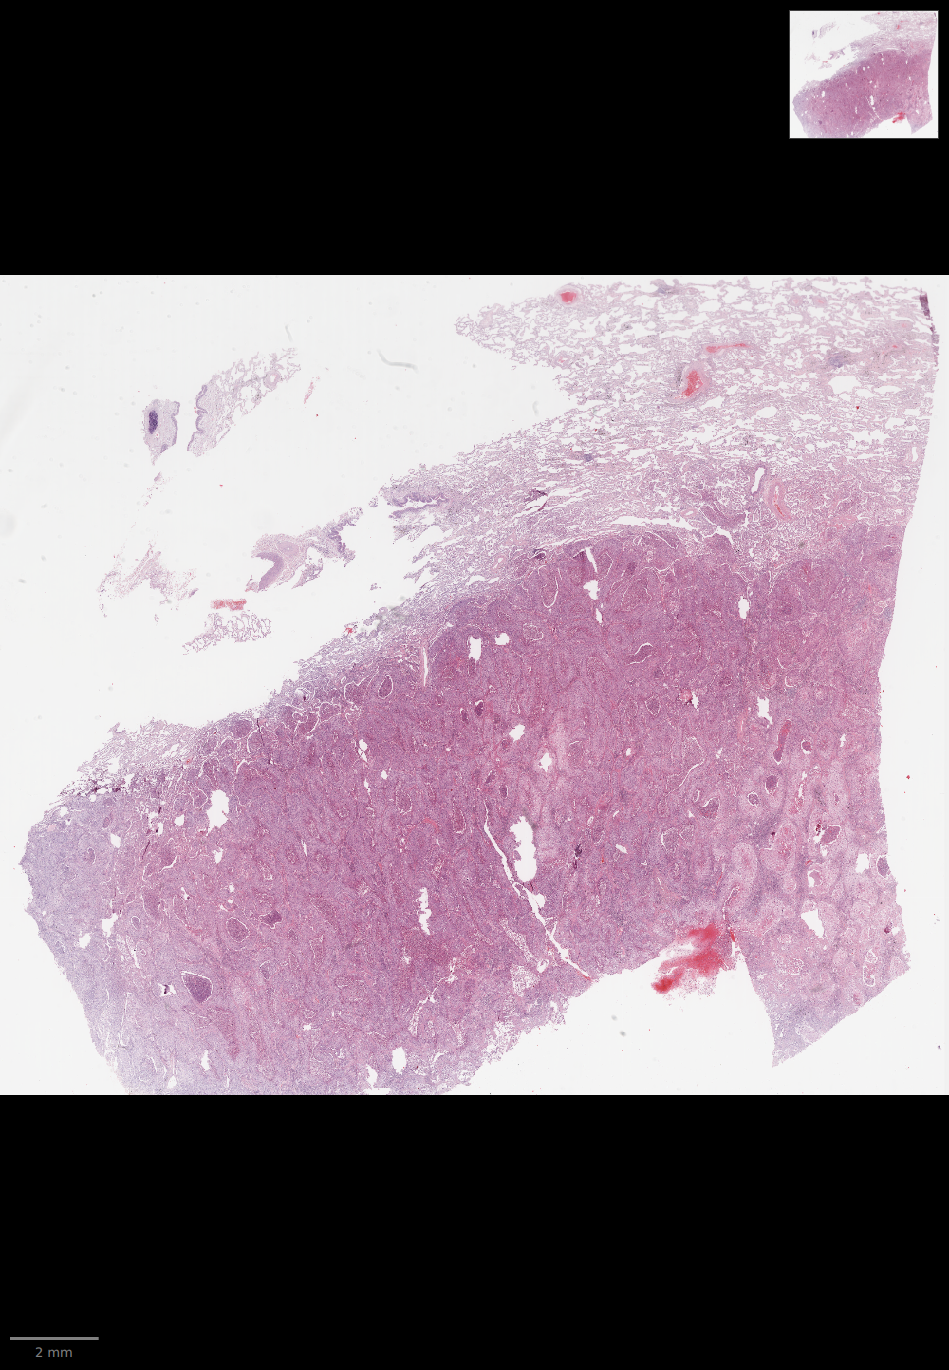
\includegraphics[width=.05\textwidth, height=.05\textheight]{./wsi7.png}}
            };
            \node[yslant=0.5, fill=blue] (cswsi\y4) at ([shift={(4*\shiftX+0.5,\y*\shiftY)}]rBase) 
            {
              {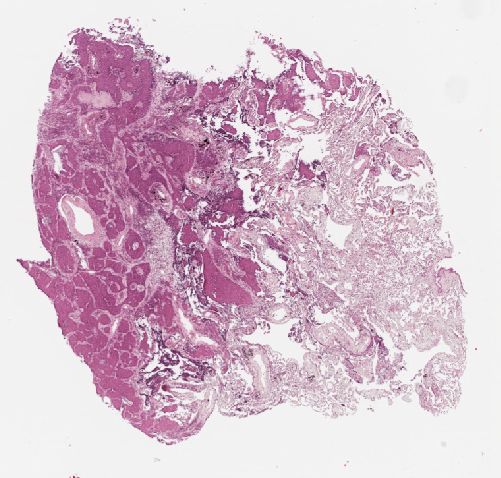
\includegraphics[width=.05\textwidth, height=.05\textheight]{./wsi8.png}}
            };
            \draw (cswsi\y1.south west) rectangle (cswsi\y4.north east) ;
            \node[anchor=north] at ([shift={(-0.8,0.5)}]cswsi\y1.west) (r3) {Batch \number\numexpr\y\relax};
            \fi
          \fi
    \end{scope}
}


\draw[->] (CS) -| ([shift={(1.5,0)}]csBase) node[above=1.5cm] {Yes, n=2} ;
\draw[->] (CS) -| ([shift={(-0.8,0)}]rBase) node[above=1.5cm] {No, randomize} ;
% \draw[->] (CS) edge node[midway, above] {No}([shift={(3.2,0.3+\shiftY)}]rBase) ;



% \foreach \x in {1,...,5}
% {
%   \node[yslant=0.5, draw] (wsi_labeled\x) at (\x,-10) 
%   {\includegraphics[width=.2\textwidth, height=.2\textheight]{./wsi\x.png}};
% }
% 
% \draw[->, thick] (3, -4.5) -- (3, -6); % Connects the midpoint below the brace to the position of the first image
% 

  %% model
  % \coordinate (base) at (0,-10);
\coordinate [below=9 of CS] (Model) {};
  \def\numLayers{5}
  \def\offset{0.2}
  \foreach \n in {1,...,\numLayers}
  {
      \pgfmathsetmacro{\shiftX}{(\numLayers - \n) * \offset}
      \pgfmathsetmacro{\shiftY}{(\numLayers - \n) * \offset / 2}

      \draw[fill=blue!30, opacity=0.9] ([shift={(\shiftX, \shiftY)}]Model) rectangle ++(.4,-2);
  }

  \node at ([shift={(2*\offset, -\numLayers*\offset - 1.5)}]Model) {Model training};

% \draw[->] (rwsi33.south)+(0,-1cm) |- (Model)+(-0.3cm,0);
% \draw[->] (rwsi33.south) -- ++(0,-1cm) |- ($(Model) + (1.5cm, 0)$) -- (Model);
% \draw[->] (cswsi33.south)+(0,-1cm) |- (Model)+(1.5cm,0) ;
\draw[->] (rwsi33.south)+(0,-1cm) |- ($(Model) + (-1.0cm,0)$);
\draw[->] (cswsi33.south)+(0,-1cm) |- ($(Model) + (2.0cm,0)$);


\end{tikzpicture}
\end{figure}

\end{document}

